To put into context, the Discrete Fourier Transform function is a simple way of extracting a finite signal's frequency content from its time domain in order to design digital filters or to convey modulated information, such as FM and OFDM.\footcite{book1_pp48_49}\\

Intuitively, this is done by correlating the entire signal sample data against a set of multiples of a given frequency for $0 \leq k \leq N$, where k is the nth frequency "bucket" (also called bin) with which the time domain signal is going to be compared against and N being number of samples.\footcite{book1_pp184_186}\footcite{book2_pp54_63}\\

Take for example the finite signal:
\[x[n] = \sin(2\pi n\times\frac{f}{f_s}), 0 \leq n < N-1 \]

Where:
\begin{itemize}
\item $f$ is the signal frequency (Hz)
\item $f_s$ is the sampling frequency (Hz)
\item $N$ is the number of samples
\end{itemize}

If we make $N = 10$, $f_s = 10$ Hz and  $f = 2$ Hz we should observe the following output:

\begin{center}
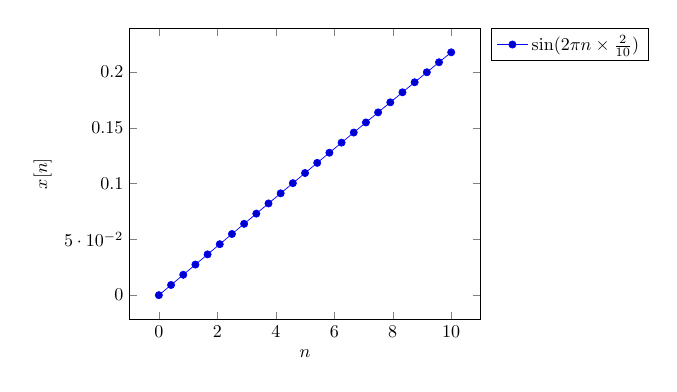
\begin{tikzpicture}[scale=0.65]
    \begin{axis}[domain=0:10,legend pos=outer north east, xlabel = {$n$},ylabel = {$x[n]$}]
    \addplot{sin(2*pi*x*(2/10))}; 
    \legend{$\sin(2\pi n \times \frac{2}{10})$}
    \end{axis}
\end{tikzpicture}
\end{center}

Each $n$ sample in this signal is compared/multiplied against a set of coefficients $h[k]$. These are complex values with real and imaginary components (in the context of DFT)\footcite{book1_pp56_60}.

In the DFT algorithm, the contents of such coefficients are made from a cosine and sine as a complex number, such that:
\[h[k] = cos\Big(\frac{2\pi kn}{N}\Big) - j\sin\Big(\frac{2\pi kn}{N}\Big)\]

Where:
\begin{itemize}
\item $k$ is the multiple of the signal frequency (bin/bucket)
\item $n$ is the nth sample with which this coefficient is going to be "compared"/multiplied against
\item $N$ is the total amount of samples in the signal
\end{itemize}

This can be simplified using Euler's formula:
\[h[k] = cos\Big(\frac{2\pi kn}{N}\Big) - j\sin\Big(\frac{2\pi kn}{N}\Big) = e^{-jnk(\frac{2\pi}{N})}\]

The process continues by accumulating the multiplication of these coefficients with the data samples in order to obtain some value that corresponds to some kind of correlation between each frequency multiple:

\[\text{\textbf{Let} } Correlation[k] \text{ be the sum of the weighted data samples},\] \[Correlation[k] = \sum_{n=0}^{n=N-1} x[n] \times h[k]\]

So, calculating for $k=0$ gives us the correlation between the entire signal data and a 0 Hz bin, which clearly is only possible in a signal with DC component.

Similarly, $k = 1$ tells us the frequency information such that: $f_k = k \times \frac{f_s}{N}$ Hz/bin $ = 1 \times \frac{10}{10}$ Hz/bin $ = 1$ Hz. If the correlation algorithm returns value $0$ or approximate, then the signal does not contain any frequency component within that $k$ bin.\footcite{book1_pp56_60}\footcite{book2_pp53}\\

In other words, it's like comparing the sample's value repeatedly against a $cosine$ and $sine$ wave tuned for the desired frequency, thus, making a different coefficient for every nth frequency bin.
For each comparison, the result is accumulated and by the end of the algorithm, we should have two results which tell us how much of the signal's frequency is contained within each multiple of a sine and cosine function.

\newpage
The higher the value is, the higher the correlation.\footcite{book1_pp62_64}\footcite{book2_pp54_63}

Finally, we have reached the conclusion that this is exactly the same expression as the DFT formula.\footcite{book1_pp56_57}\footcite{book2_pp50}
\[Correlation[k] = \sum_{n=0}^{n=N-1} x[n] \times  e^{-jnk(\frac{2\pi}{N})}\]
\[\Leftrightarrow\]
\[X[k] = \sum_{n=0}^{n=N-1}x[n]\times e^{-jnk(\frac{2\pi}{N})}\]

Lastly, it's important to note that it is common to use the magnitude of the resultant real and imaginary values as the desired output of the DFT\footcite{book1_pp58}. The real and imaginary components could however give more insight into the signal's properties, such as phase.\\

This calculation is easily done by first converting the exponent into its trigonometric form (Euler's formula again), followed by a sum of the two complex components squared:
\[|X[k]| = \sqrt{\Bigg[\sum_{n=0}^{n=N-1}x[n]\times\cos\Big(\frac{2\pi kn}{N}\Big)\Bigg]^2 + \Bigg[\sum_{n=0}^{n=N-1}x[n]\times -j\sin\Big(\frac{2\pi kn}{N}\Big)}\Bigg]^2\]

\newpage
\paragraph{}
In regards to the report, this first section will apply the DFT theory that was just described to three different signals:
\begin{itemize}
\item A $2$ kHz sine wave with amplitude of $A = 10$
\item A mix of three sine waves with frequencies $500$ Hz, $1$ kHz and $2$ kHz respectively and amplitudes of $A = 10$
\item A square wave with amplitude $0 \leq A \leq 20$
\end{itemize}

All signals are composed of $N = 256$ samples and these are sampled at a frequency of $f_s = 15$ kHz.\\

Finally, the DFT function will be done with resolution of $k = 256$ points and this output will be displayed in the logarithmic scale by calculating $20\log_{10}(Spectrum[k])$.

%%%%%%%%%%%%%%%%%%%%%%%%%%%%%%%%%%%%%%%%%%%%%%%%%%%%%%%%%%%%%%%%%%%%%%%%%%%%%%%%%%%
%%%%%%%%%%%%%%%%%%%%%%%%%%%%%%%%%%%%%%%%%%%%%%%%%%%%%%%%%%%%%%%%%%%%%%%%%%%%%%%%%%%
%%%%%%%%%%%%%%%%%%%%%%%%%%%%%%%%%%%%%%%%%%%%%%%%%%%%%%%%%%%%%%%%%%%%%%%%%%%%%%%%%%%
\newsubsection{1.A) 256 DFT on a sine wave}

The first signal to analyse is a simple sinusoidal. Its expression:
\[x(t) = 10\sin(2\pi t\times 2000)\] 

Since the DFT is a discrete transform, the signal must be sampled first by dividing the frequency\footcite{book1_pp55_56}.
\[x[n] = 10\sin\Big(2\pi n\times\frac{2000}{15000}\Big)\]

Which results in the following graph:
\showplot{Q1A1}{Sine wave input [f = 2 kHz $f_s = 15$ kHz amplitude = 10 and 256 samples]}

This wave form was generated with the C function below:
\lstinputlisting[firstline=42, lastline=55, caption=Function: create\_sinewave() - dsp\_functions.c]{../Visual-Studio-Project/NG4S804_Assignment1/NG4S804_Assignment1/dsp_functions.c}

\newpage
Its usage:
\lstinputlisting[firstline=18, lastline=26, gobble=4, caption=Usage: allocating a sine wave - question1\_a.c]{../Visual-Studio-Project/NG4S804_Assignment1/NG4S804_Assignment1/question1_a.c}

After passing the signal through the DFT algorithm, we are presented with its single sided spectrum (linear scale):
\showplot{Q1A2SSB}{DFT spectrum [256 points Single-Sideband (SSB)] of sine wave [f = 2 kHz $f_s = 15$ kHz amplitude = 10 and 256 samples]}\\
(\textbf{\underline{Note}} that this is the last time a spectrum with linear scale is shown. The reason is due to the report's requirements. In addition, all spectrums will be Single Sideband (SSB) \underline{unless} it is specified otherwise.)

\newpage
In the logarithmic scale:
\showplot{Q1A3SSB}{DFT spectrum [256 points SSB] of sine wave [f = 2 kHz $f_s = 15$ kHz amplitude = 10 and 256 samples] dB}

The results were produced using the DFT function below:
\lstinputlisting[firstline=4, lastline=40, caption=Function: DFT() - dsp\_functions.c]{../Visual-Studio-Project/NG4S804_Assignment1/NG4S804_Assignment1/dsp_functions.c}

\newpage
And its usage:
\lstinputlisting[firstline=70, lastline=74, caption=Usage: converting the input into the frequency domain - question1\_a.c]{../Visual-Studio-Project/NG4S804_Assignment1/NG4S804_Assignment1/question1_a.c}

Also note $convert\_to\_log\_scale()$'s function implementation:
\lstinputlisting[firstline=102, lastline=113, caption=Function: convert\_to\_log\_scale() - dsp\_functions.c]{../Visual-Studio-Project/NG4S804_Assignment1/NG4S804_Assignment1/dsp_functions.c}

\paragraph{}
Needless to say, Figure 3 clearly shows a peak at $k = 34$ which can be seen at the top of the horizontal axis. Even though the plot already displays the frequency information for that specific $k$, it's still important to show how this was calculated\footcite{book2_pp53}:
\[f_k = \frac{k\times f_s}{N}\]

Where:
\begin{itemize}
\item $N$ is the sample count ($N = 256$)
\item $f_s$ the sampling frequency ($f_s = 15$ kHz)
\end{itemize}

So, in this case, if the peak occurs at $k = 34$, then the signal frequency must be:
\[f_k = \frac{34\times 15000}{256} \approx \mathbf{1992.2}\textbf{ Hz}\]

And indeed the input signal is composed of a $2000$ Hz sinusoidal, which clearly indicates that the C function $DFT()$ is implemented correctly.\\

Also, note the error between the expected value and the returned value, which is

$\mathbf{error = 2000 \textbf{ Hz } - 1992.2 \textbf{ Hz } = \color[HTML]{FE0000}7.8}$ \textbf{Hz}.
This is one of the trade offs of treating analogue signals as finite discrete data.

Since we have  $k = 256$ bins, with frequency ranges of $[0, 15000]$ Hz, and each $k$ being a multiple of $f_k = \frac{f_s}{N} = \frac{15000}{256} = 58.59$ Hz, we notice that some information is going to be lost.\\

This is called Spectral leakage.\footcite{book2_pp71_80}

\newpage
In short, we lack the ability to determine the frequency content below $58.59$ Hz of resolution because the bin count is simply too small to represent an entire range of $15$ kHz. If we wanted a resolution of 1, then we would increase the DFT point count to $f_s = 15000$, but even then we would not be able to process frequencies with resolution finer than $1$ Hz. (e.g. $0.5$ Hz, $0.25$ Hz or $0.125$ Hz.)\\

In addition, the C program defines $k$ as an integer value, which means this variable can only hold natural numbers (due to the fact that arrays can only be indexed with integers) and therefore the only possible values in this case are:
\[\text{if } k=34 \text{ then: } f_k = \frac{34\times 15000}{256} = 1992.2 \text{Hz}\]
and
\[\text{if }k=35 \text{ then: } f_k = \frac{35\times 15000}{256} = 2050.78 \text{Hz}\]
Clearly the result for $k = 35$ goes way beyond $2000$ Hz.\\

If we had the capacity to calculate $k$ as a decimal value, then the real value of $k$ for this signal should be: $k = \frac{f_k\times N}{f_s} = \frac{2000\times 256}{15000} = 34.13$. However, the value was rounded down to $k = 34$, thus we obtain the error of $7.8$ Hz.\\

By this logic, we conclude that an infinite amount of $k$ bins would be the same as having the ability to process the signal's frequency information at any possible harmonic, with $\delta f$ for every $k$ being practically 0.\\

(hint: this infinite process is literally just a continuous Fourier Transform.\footcite{book1_pp55_56})

%%%%%%%%%%%%%%%%%%%%%%%%%%%%%%%%%%%%%%%%%%%%%%%%%%%%%%%%%%%%%%%%%%%%%%%%%%%%%%%%%%%
%%%%%%%%%%%%%%%%%%%%%%%%%%%%%%%%%%%%%%%%%%%%%%%%%%%%%%%%%%%%%%%%%%%%%%%%%%%%%%%%%%%
%%%%%%%%%%%%%%%%%%%%%%%%%%%%%%%%%%%%%%%%%%%%%%%%%%%%%%%%%%%%%%%%%%%%%%%%%%%%%%%%%%%
\newsubsection{1.B) 256 DFT on a mix of three sine waves}
In this task the same approach is used for analysing a signal that is similar to the previous exercise. This time three sinusoids with different harmonics are to be added together.
\[x_1(t) = 10\sin(2\pi t \times 500) \text{ , f = 500 Hz}\]
\[x_2(t) = 10\sin(2\pi t \times 1000) \text{ , f = 1000 Hz}\]
\[x_3(t) = 10\sin(2\pi t \times 2000) \text{ , f = 2000 Hz}\]
\[x_{mix}(t) = x_1(t) + x_2(t) + x_3(t)\]
\[\text{All 3 input signals have amplitude = 10}\]

After discretization (with the sampling frequency being $f_s = 15$ kHz):
\[x_{mix}[n] =10\bigg[\sin\Big(2\pi n \times \frac{500}{15000}\Big) + \sin\Big(2\pi n \times \frac{1000}{15000}\Big) + \sin\Big(2\pi n \times \frac{2000}{15000}\Big)\bigg]\]

And this results in the following output:
\showplot{Q1B1}{Mixed sine wave input [f = 0.5 kHz + 1 kHz + 2 kHz $f_s = 15$ kHz amplitude = 10 and 256 samples]}

\newpage
The generator function uses the function found in the listing \underline{\textbf{$Code$ $1$}} followed by a simple addition with a for loop:
\lstinputlisting[firstline=21, lastline=29, caption=Usage: creating and mixing 3 sine waves - question1\_b.c]{../Visual-Studio-Project/NG4S804_Assignment1/NG4S804_Assignment1/question1_b.c}

Finally, the frequency spectrum:
\showplot{Q1B13SSB}{DFT spectrum [256 points SSB] of three mixed sine waves [f = 0.5 kHz + 1 kHz + 2 kHz amplitude = 10 and 256 samples] dB}

Again, we clearly see the peaks of the three input signals at their correct frequency values. The $k$ bins for all three peaks are (with approximation to the nearest integer):
\begin{table}[!hb]
\centering
\begin{tabular}{|c|c|c|c|c|c|}
\hline
\textbf{Peak \#} & \textbf{k} & \textbf{expected k}                      & \textbf{$f_k$ (Hz)}                        & \textbf{expected $f_k$ (Hz)} & \textbf{error (Hz)}          \\ \hline
1                & 9          & $k = \frac{500\times 256}{15000} = 8.53$ & $f_k = \frac{9\times 15000}{256} = 527.34$ & 500                          & {\color[HTML]{FE0000} 27.34} \\ \hline
2                & 17         & 17.1                                     & 996.1                                      & 1000                         & {\color[HTML]{FE0000} 3.9}   \\ \hline
3                & 34         & 34.13                                    & 1992.2                                     & 2000                         & {\color[HTML]{FE0000} 7.8}   \\ \hline
\end{tabular}
\caption{Peaks of the 256 DFT - Mixed sine wave}
\label{265DFT-mixsine}
\end{table}

%%%%%%%%%%%%%%%%%%%%%%%%%%%%%%%%%%%%%%%%%%%%%%%%%%%%%%%%%%%%%%%%%%%%%%%%%%%%%%%%%%%
%%%%%%%%%%%%%%%%%%%%%%%%%%%%%%%%%%%%%%%%%%%%%%%%%%%%%%%%%%%%%%%%%%%%%%%%%%%%%%%%%%%
%%%%%%%%%%%%%%%%%%%%%%%%%%%%%%%%%%%%%%%%%%%%%%%%%%%%%%%%%%%%%%%%%%%%%%%%%%%%%%%%%%%
\newsubsection{1.C) 256 DFT on a square wave}
The third and last signal is a square wave with frequency of 500 Hz and amplitude from 0 to 20.

\paragraph{}
Since a square wave is composed of an infinite set of sinusoids\footcite{book1_pp49} , creating one with a C program becomes much less practical and intuitive as opposed to generating a single sine wave with the $sin()$ function. In this case, the program tries to approximate the square wave with the algorithm:
\[x[n] = \begin{cases} 20, & \mbox{if } sin(2\pi n \times \frac{500}{15000}) \geq 0 \\ 0, & \mbox{if } sin(2\pi n \times \frac{500}{15000}) < 0 \end{cases}\]
\showplot{Q1C1}{Square wave input [f = 0.5 kHz $f_s$ = 15 kHz amplitude = 20 and 256 samples]}

\newpage
The code for it:
\lstinputlisting[firstline=57, lastline=70, caption=Function: create\_squarewave() - dsp\_functions.c]{../Visual-Studio-Project/NG4S804_Assignment1/NG4S804_Assignment1/dsp_functions.c}

And how to use it:
\lstinputlisting[firstline=18, lastline=19, caption=Usage: allocating a square wave - question1\_c.c]{../Visual-Studio-Project/NG4S804_Assignment1/NG4S804_Assignment1/question1_c.c}

Which gives the frequency spectrum:
\showplot{Q1C3SSB}{DFT spectrum [256 points SSB] of square wave [f = 0.5 kHz $f_s$ = 15 kHz amplitude = [0, 20] and 256 samples] dB}

After analysing the output, we quickly come to the conclusion that there is not only signal being fed through the input, but there are 8 apparent signals, one of them being purely DC at 0 Hz where $k = 0$ (which will be ignored while calculating $f_k$). As can be seen, this experiment proves that a square wave is indeed just a mix of infinite sinusoids with different frequencies, as described by the Fourier Series.

\newpage
\paragraph{}
According to the plot, each peak is expected to be found at frequencies 0, 500, 1500, 2500, 3500, 4500, 5500 and 6500 Hz. The measured $k$ bins are therefore:
\begin{table}[!hb]
\centering
\begin{tabular}{|c|c|c|c|c|c|}
\hline
\textbf{Peak \#} & \textbf{k} & \textbf{expected k}                      & \textbf{$f_k$ (Hz)} & \textbf{expected $f_k$ (Hz)} & \textbf{error (Hz)}          \\ \hline
1                & 9          & $k = \frac{500\times 256}{15000} = 8.53$ & $f_k = \frac{9\times 15000}{256} = 527.34$                 & 500                          & {\color[HTML]{FE0000} 27.34} \\ \hline
2                & 26         & 25.6                                     & 1523.44             & 1500                         & {\color[HTML]{FE0000} 23.44} \\ \hline
3                & 43         & 42.67                                    & 2519.53             & 2500                         & {\color[HTML]{FE0000} 19.53} \\ \hline
4                & 60         & 59.73                                    & 3515.63             & 3500                         & {\color[HTML]{FE0000} 15.63} \\ \hline
5                & 77         & 76.8                                     & 4511.72             & 4500                         & {\color[HTML]{FE0000} 11.72} \\ \hline
6                & 94         & 93.87                                    & 5507.81             & 5500                         & {\color[HTML]{FE0000} 7.81}  \\ \hline
7                & 111        & 110.93                                   & 6503.9              & 6500                         & {\color[HTML]{FE0000} 3.91}   \\ \hline
\end{tabular}
\caption{Peaks of the 256 DFT - Square wave}
\label{265DFT-squarewave}
\end{table}

Also it's important to notice that the highest peak can be found at $k = 9$. This means that despite the fact that this specific square wave is composed of 7 main harmonics (excluding DC), we are still able to determine the actual desired frequency of the original signal, which is clearly indicated by the much larger magnitude at $k = 9$.